\chapter{Testing}

During this project many different testing methods were performed. This section will discus the testing that has been carried out during the different stages of the project.

\section{Unit Testing}

\subsection{JavaEE}
While developing we placed all back-end code within service classes. This would allow unit tests to be performed. However in some cases the use of mock class would also be required to mock the classes accessing the database. 
	
In order to mock the behaviour of the facade classes Mockito\cite{Mockito} has been used. All facade methods which the class under test calls are mocked. 

\begin{figure}[H]
\begin{center}
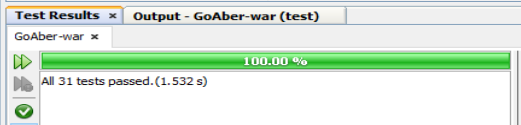
\includegraphics[scale=0.6]{images/testing/UnitTestsJavaEE.png} 
\caption{JavaEE unit tests.}
\label{fig:testing_vsBuild}
\end{center}
\end{figure}

\subsection{.NET}
This initial plan was to perform unit testing in the same manor as JavaEE. Unfortunately, the .NET service class are not as easily testable. Nearly all of the code in these service classes contain SQL. When running the unit tests the database is inaccessible, therefore only code that does not access the database can be tested. 

To get around the database access issues we considered using of Moq \cite{Moq}. However, this would cause considerable change to the code as interfaces would be required for all classes being mocked. 

Using unit testing the controllers was also considered, but again mocking classes would have to be used to stop these from accessing database code. As cucumber testing was already being used, little would be gain by adding controller tests. The cucumber tests would allow the checkout that the correct views and database is presented to the user.

\begin{figure}[H]
\begin{center}
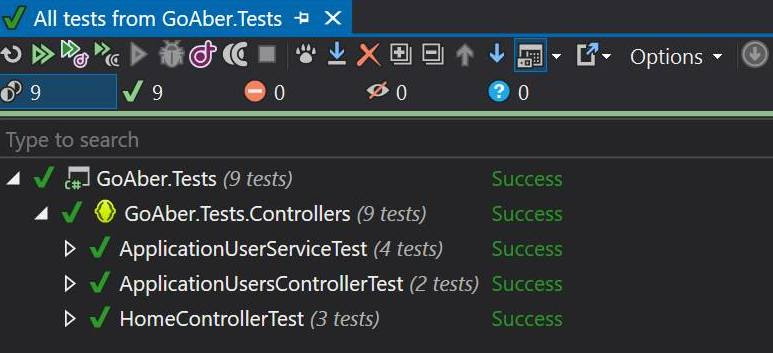
\includegraphics[scale=0.3]{images/testing/unitTestsNET.jpg} 
\caption{.NET unit tests}
\label{fig:testing_unitTestNET}
\end{center}
\end{figure}

\section{Continuous Integration}

\subsection{Automated Continuous Integration}
\subsubsection{.NET}

Visual Studio Online allows continuous integration to be performed automatically. This allowed us to test that our project builds correct after a developer has integrated their work with the main development branch.

Due to a the limited time of build time available, during the first 4 sprints the automatic build was only triggered when a merge to master occurred. This merge happened at the end of every sprint. During the latter stages of the project the automatic build was set to the ``develop" branch. This allowed us to discover bugs more quickly as the final parts of the project came together.

As shown in figure~\ref{fig:testing_vsBuild} some builds failed. When a build failed an email was automatically sent out to all developers. This allowed the bug to be quickly resolved and the build to be re-ran.


\begin{figure}[H]
\begin{center}
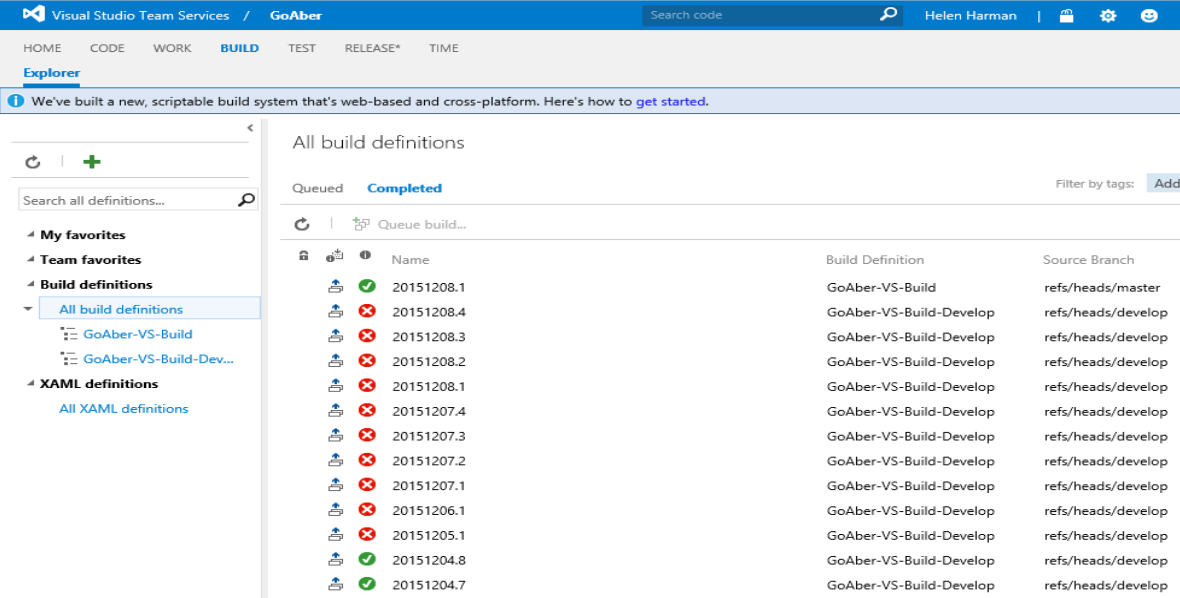
\includegraphics[scale=0.3]{images/testing/builds.png} 
\caption{Selection of builds that have been run during the project.}
\label{fig:testing_vsBuild}
\end{center}
\end{figure}

The summary information on the build (figure~\ref{fig:testing_vsBuildExample}) allowed us to view how long the build look at if there are any issues. For example warnings about unused variables.

\begin{figure}[H]
\begin{center}
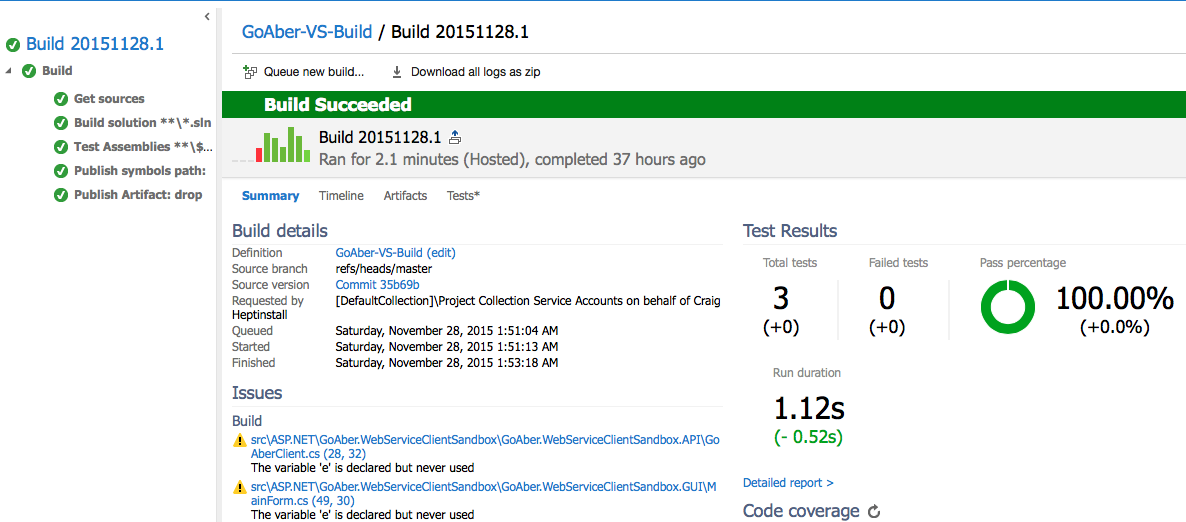
\includegraphics[scale=0.3]{images/testing/ExampleBuild.png} 
\caption{Example of a build that has been performed.}
\label{fig:testing_vsBuildExample}
\end{center}
\end{figure}

\subsubsection{JavaEE}
Consideration was given to changing the JavaEE project into a Maven project. This would allow Visual Studio Online to build the project. However, it was not discovered until a considerable amount of work had gone into the project that Visual Studio Online used Maven. A decision was made that changing to Maven at this stage would take too much time away from development, and the manual integration testing was providing a sufficient method of integration testing.


\subsection{Manual Integration Testing}
Throughout the first 4 sprints of the project no developer was allowed to push to the develop branch unless two other group members had tested and reviewed their code. This was enforced using Visual Studio Online. Due to the number of these pull request being made, this changed to one developer in order to speed up the process.

\begin{figure}[H]
\begin{center}
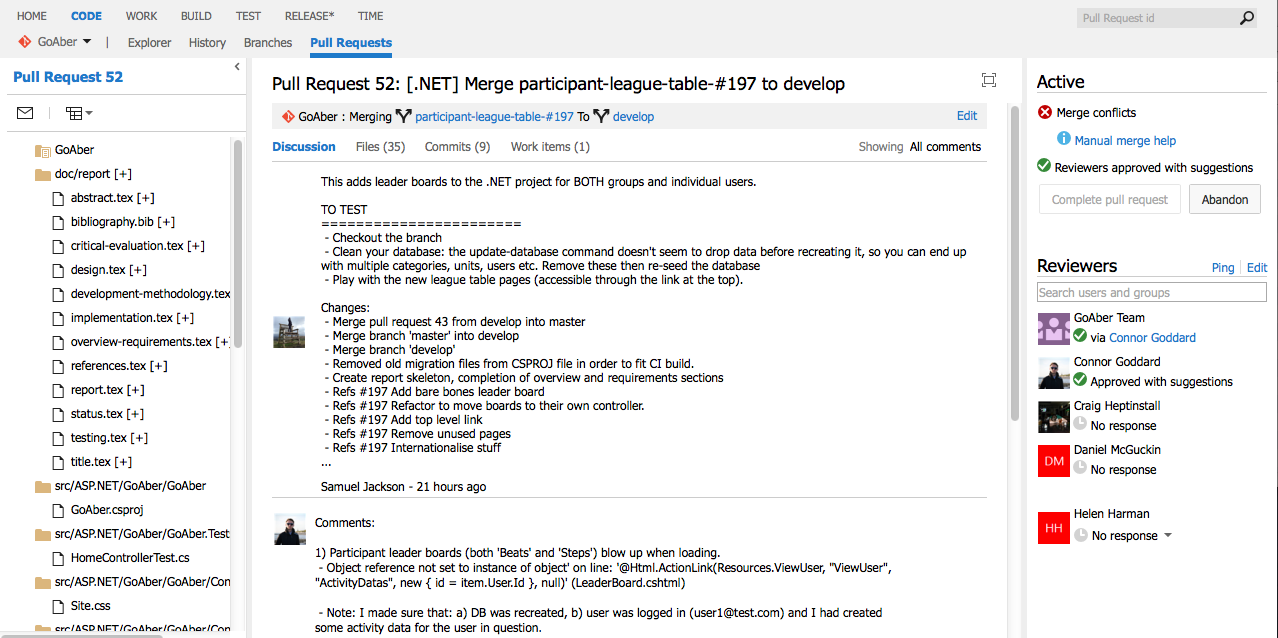
\includegraphics[scale=0.3]{images/testing/PullRequest.png} 
\caption{Example of a pull request}
\label{fig:testing_pullRequest}
\end{center}
\end{figure}

For a pull request to be approved the project must build and the tasks stated by the creator should work as stated within the request. Within each pull request steps on how to test the functionality have been provided. An example of this is shown in figure~\ref{fig:testing_pullRequest}.

As well as checking the functionality the reviewer also performed a small code review. This would encourage the use of clean commented code, which follows the MVC design pattern.

As well as finding many bugs, this also allowed multiple members of the group to learn about how a requirement of the system had been implemented.

\section{User Interface Testing}

To test the user interface SpecFlow \cite{SpecFlow} was used. SpecFlow allows the creation of behaviour driven test that are written in plain English scenarios contained within feature files. These scenarios (figure~\ref{fig:testing_cucumberScenarios}), along with some step definitions (figure~\ref{fig:testing_cucumberCodeSteps}) allow interactions with the user interface to be performed. 

\begin{figure}[H]
\begin{center}
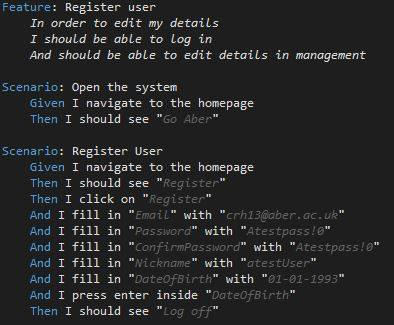
\includegraphics[scale=0.6]{images/testing/cucumberScenarios.jpg} 
\caption{Cucumber test scenarios}
\label{fig:testing_cucumberScenarios}
\end{center}
\end{figure}

\begin{figure}[H]
\begin{center}
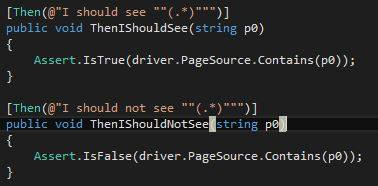
\includegraphics[scale=0.6]{images/testing/cucumberCodeSteps.jpg} 
\caption{Cucumber steps}
\label{fig:testing_cucumberCodeSteps}
\end{center}
\end{figure}

PhantomJS \cite{PhantomJS} allowed us to run the tests without opening an internet browser. This will allow the tests to be ran by our continuous integration server. Selenium web driver is used to select and control the web browser.

Tests to check that no invalid data can be entered into the forms are performed. This includes boundary checks, valid type checks and valid format (e.g. email format) checks. The results of the tests are shown in figure~\ref{fig:testing_cucumberPassedTests}.

The steps (shown in figure~\ref{fig:testing_cucumberCodeSteps}) only have to be written once. These tests interact with the HTML in the web browser, therefore, they do not care about the underlying technologies. By just changing a URL these test can be used for both the JavaEE and .NET projects. 

\begin{figure}[H]
\begin{center}
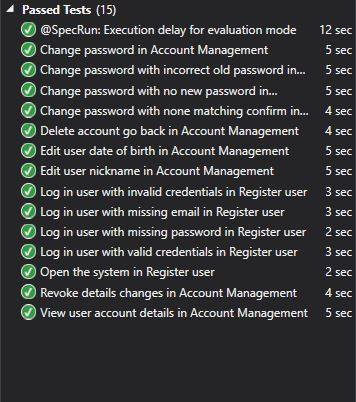
\includegraphics[scale=0.6]{images/testing/cucumberPassedTests.jpg} 
\caption{Cucumber test results}
\label{fig:testing_cucumberPassedTests}
\end{center}
\end{figure}

Using the SpecFlow library has also resulted in the automated creation of testing statistics similar to that of standard cucumber. Shown in figure ~\ref{fig:testing_html_results} is the result from running tests, where a useful html page has been created. The page shows run time, number of tests in each feature, alongside descriptions of each of the tests, and reasons for any failures. As the figure shows, no tests failed at the stage of completion of testing. Where failures were found during the testing process, fixes were completed to the application.

\begin{figure}[H]
\begin{center}
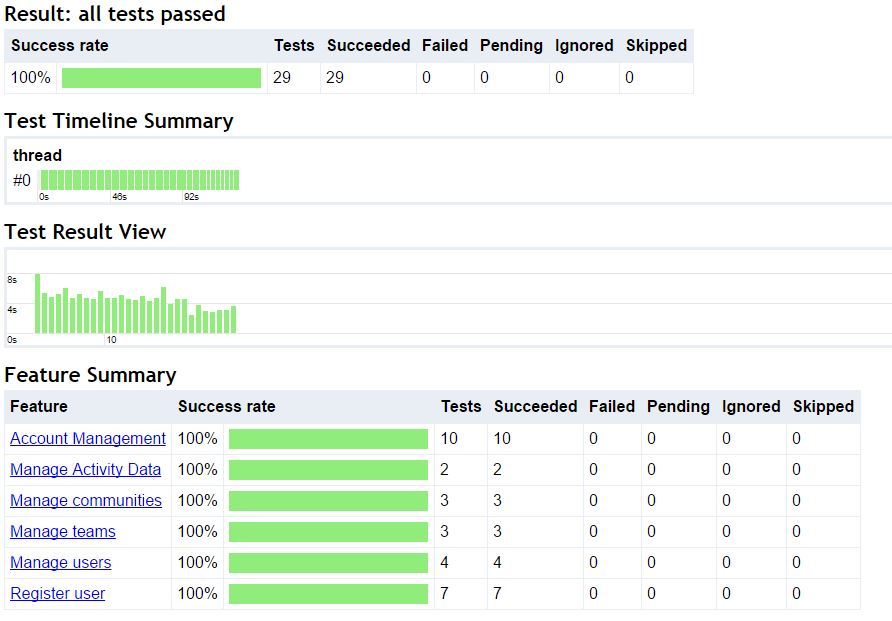
\includegraphics[scale=0.6]{images/testing/specflowResults.jpg} 
\caption{Cucumber test results, generated inside HTML pages}
\label{fig:testing_html_results}
\end{center}
\end{figure}

\section{SOAP Communication}
To test that 3rd-party applications can send our application activity data a second application was created. This second application just sends activity data to our main application. 

\subsection{.NET}
For .NET a GUI application was created to allow the entry of an authorisation token (Shown in figure~\ref{fig:testing_authTokenNet}). This token is sent to the main application along with the activity data. The main application will check the validity of the token before saving the activity data to the database. The activity data will be associated with the user that is currently logged into the application.

\begin{figure}[H]
\begin{center}
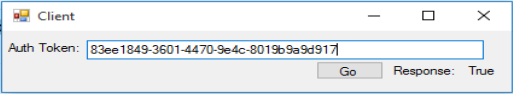
\includegraphics[scale=0.3]{images/testing/clientAuthTokenNET.png} 
\caption{The .NET SOAP client application.}
\label{fig:testing_authTokenNet}
\end{center}
\end{figure}


Unit tests have also been added to the project to test that the data can be sent and the valid return value is received. (Shown in figure~\ref{fig:testing_SoapUnitTestsNET}.)

\begin{figure}[H]
\begin{center}
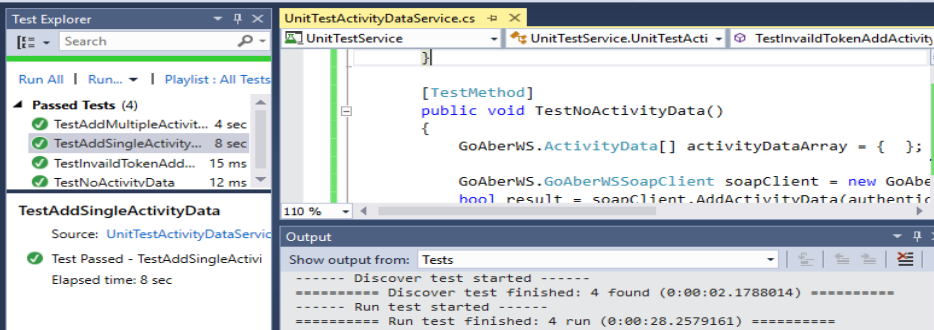
\includegraphics[scale=0.3]{images/testing/SoapUnitTestsNET.png} 
\caption{Unit tests for the SOAP operations in the .NET project.}
\label{fig:testing_SoapUnitTestsNET}
\end{center}
\end{figure}


\subsection{JavaEE}

The JavaEE SOAP test is a command line application which, like the .NET application, allows the user to enter an authorisation token. When running this application the user does not need to be logged in. Which users account to added the activity data too is specified in the request. Unit tests have also been added to this project.

\begin{figure}[H]
\begin{center}
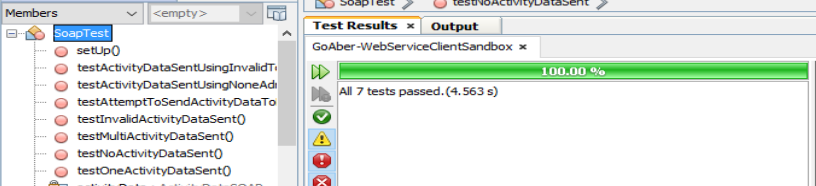
\includegraphics[scale=0.3]{images/testing/SoapUnitTestsJavaEE.png} 
\caption{Unit tests for the SOAP operations in the JavaEE project.}
\label{fig:testing_SoapUnitTestsJavaEE}
\end{center}
\end{figure}


\section{Cross Browser Compatibility}

Throughout the project the applications were tested on multiple browsers this includes Chrome, Safari, Internet Explore 11, Edge and Opera. Both application should work on all modern browsers.

\section{Community Communication}

To test that a community could send a challenge to a different community, we ran instances of the JavaEE and .NET projects on different computers. These tests involved checking that both instances could send and receive challenges, and that the community which started the challenge sent the results to all other communities.

